\section{倾角影响}
\label{sec:3.2}

本节从计算射线在某些理想条件下的旅行时间来开始地震旅行时间对炮检距依赖关系的
研究。

\subsection{平面反射面情形下的剖面与道集}
\label{sec:3.2.1}

对于反射资料,最简单情况就是如图\ref{fig:ofs/twopoint}所示的一个水平反射分界面。正如所预料的,
零炮检距剖面酷似地层模型。共中心点道集的时距曲线是双曲线,其渐近线是直线,该直线
的斜率等于速度$v_1$的倒数。最基本的数据处理称为共深度点叠加。即CDP叠加。处理中,
将典中心点道集(CMP)的所有记录道进行时差校正,使时距曲线拉平成为直线,然后彼
此相加,所得结果酷似一个零炮检距记录道。所有这些记录道集合起来,就叫作共深度点叠
加剖面。实际上,总是把CDP叠加剖面当作是一个零炮检距剖面来加以解释和进行偏移.
在本节中,我们将要讨论如何避免采用这种流行的、过于简单化的假设。

\begin{figure}[H]
\centering
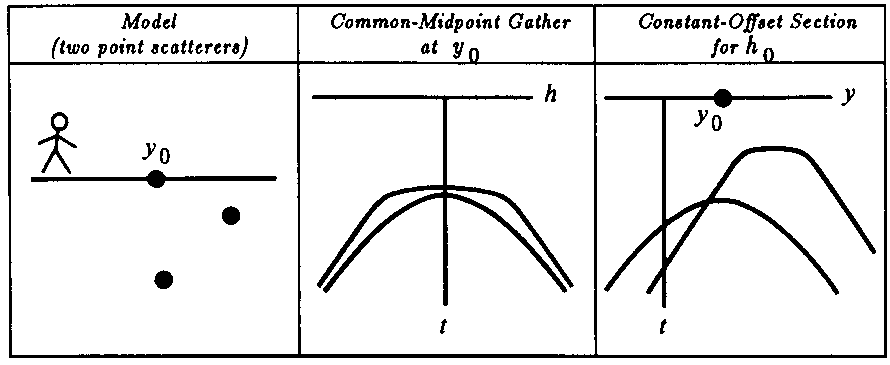
\includegraphics[width=0.65\textwidth]{ofs/twopoint}
\caption[twopoint]{最简单的地层模型}
\label{fig:ofs/twopoint}
\end{figure}

其次一种最简单情形是具有平面反射面,但方向为垂直而非水平。这种情形并不是典型
情形,不过因为地层倾角的影响在极端情形下更易被理解,所以讨论中还是包括了这种情
形。现在,波是沿着空气与大地的分界面传播。为避免混乱,可令反射面以很小的角度偏离
垂直方向,如图\ref{fig:ofs/vertlay}所示。

\begin{figure}[H]
\centering
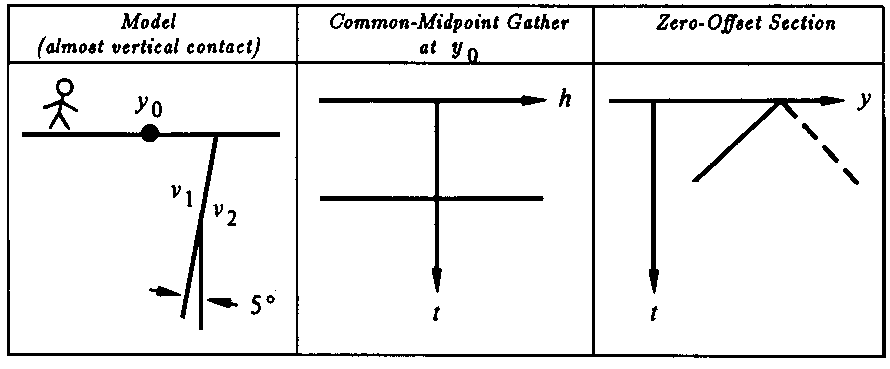
\includegraphics[width=0.65\textwidth]{ofs/vertlay}
\caption[vertlay]{将近垂直的反射面以及相应的道集和剖面}
\label{fig:ofs/vertlay}
\end{figure}

图\ref{fig:ofs/vertlay}表明,旅行时间并不随炮检距之改变而变化。当炮点与检波点彼此逐渐分离
时,旅行时间并不随之增加,看起来似乎有些自相矛盾,解释这种矛盾的关键就在于:保
持恒定不变的是中心点,而不是炮点。在炮检距增大时,炮点虽越易远离该反射面而检波点
却更接近于该反射面,因而,在一个射线路程上的时间减小了,在另一个路程上的时间却增
大了。

平面反射面可以具有位于水平与垂直之间的任何倾角,从而其共中心点道集应处于图
\ref{fig:ofs/twopoint}所示共中心点道集与图\ref{fig:ofs/vertlay}那种共中心点道集之间。
图\ref{fig:ofs/vertlay}内的零炮检距剖面是一条直线,原来它就是双曲线族的渐近线,该渐近线的斜率就等于速度$v_1$的倒数。

\subsection{倾斜层}
\label{sec:3.2.2}
